\documentclass{csfourzero}

\title{CS4040 Example Report Structure}
\author{Timothy J.\ Norman}
\date{\today}
% A useful package to support on-line references
\usepackage{url}
\usepackage{natbib}

\bibliographystyle{plain}

\begin{document}
\maketitle

\section{Introduction}
\label{sec:intro}

The aim of the introduction is to say what you are going to investigate in the report and why it
  is interesting.

Guide length: 250 words.

\section{Background and related work}
\label{sec:lit}

A review of related work \cite{Stallings2010,cryptowiki}.

Guide length: 500 words.

\section{Research question}
\label{sec:rq}

Given the problem context (Section~\ref{sec:intro}) and background
(Section~\ref{sec:lit}), you should now be in a position to present
what you have investigated. \textbf{Pose this as a question.}

Then you should present your approach to addressing this
question.

Guide length: 500 words.

\section{Experimental Design}
\label{sec:exp}

What are your hypotheses? How are you going to test them? What is your
target population? What are your datasets; i.e.\ your sample of the
target population. What are the dependent and independent variables?

Guide length: 500 words.

\section{Results}
\label{sec:results}

Present the results. A good way to organise this is via subsections
for each hypothesis you tested. Include graphs of results
(e.g.\ Figure~\ref{fig:data}), tests of significance, etc. If you have
negative results, include them. A negative results is just as
informative and useful as a positive one, sometimes more so.

\begin{figure}
\centerline{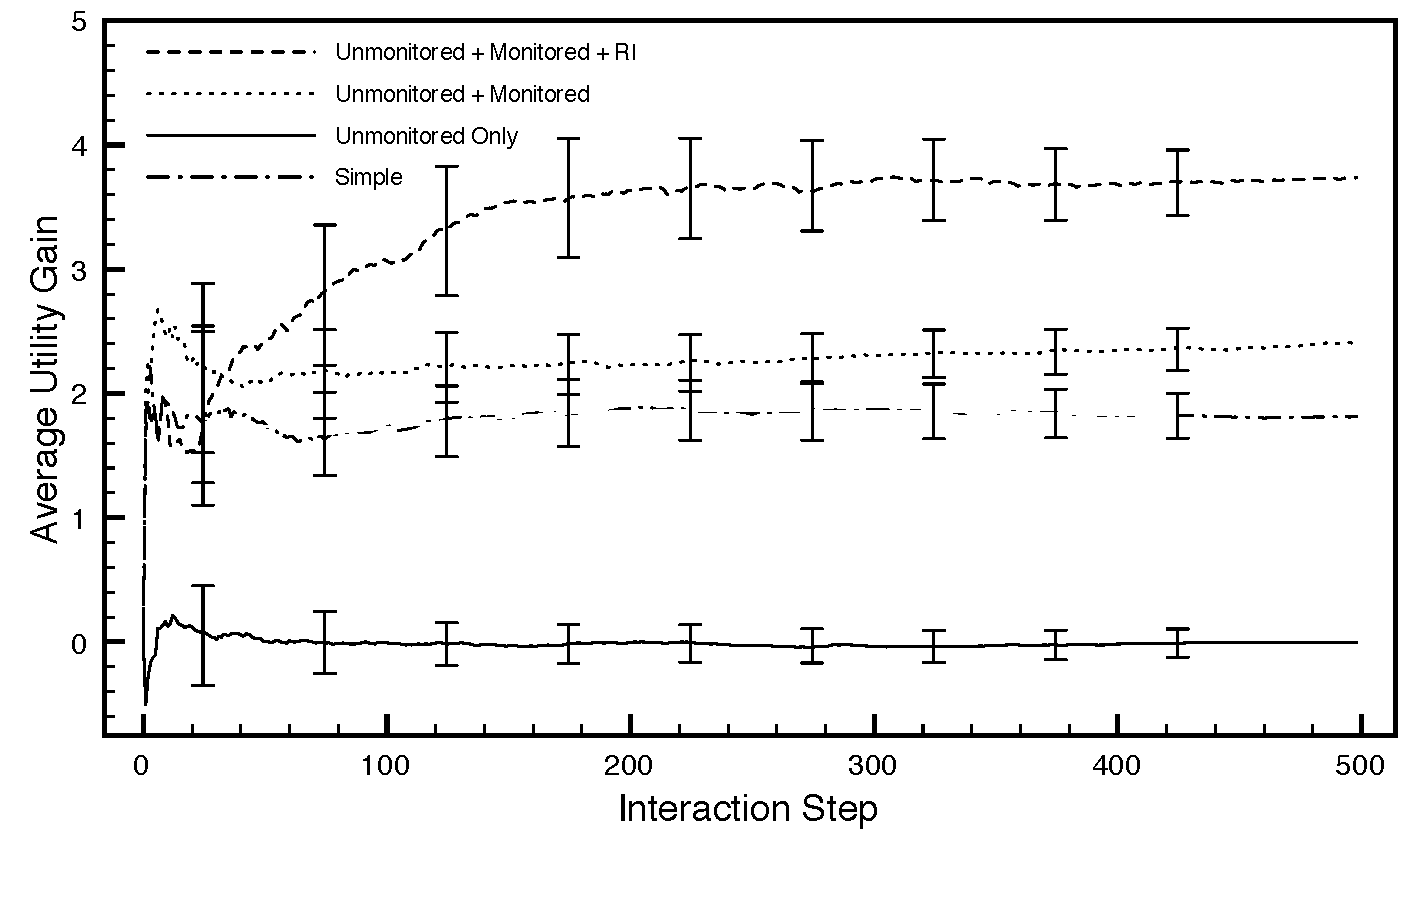
\includegraphics[width=5in]{basic-data-errors}}
\caption{Some results.}\label{fig:data}
\end{figure}

Guide length: 500 words.

\section{Discussion}
\label{sec:discuss}

What do the results say? What have you learned from the
experiments? Have you identified a correlation between variables, or
causation? What are the limitations of what you've done? What further
experiments might be of benefit?

Guide length: 400 words.

\section{Conclusion}
\label{sec:conc}

What have you done and why? What have you shown through your
experiments?

Guide length: 100 words.

\bibliography{myrefs}

\end{document}
